\documentclass[11pt]{article}
\usepackage[margin=2.2cm]{geometry}
\usepackage{amsmath,amssymb}
\usepackage{booktabs}
\usepackage{graphicx}
\usepackage{enumitem}
\usepackage{xcolor}
\usepackage[colorlinks=true,linkcolor=blue!50!black,urlcolor=blue!50!black]{hyperref}
\setlist{nosep,leftmargin=*}
\setlength{\parskip}{4pt}
\setlength{\parindent}{0pt}
\newcommand{\ms}{\,\mathrm{m/s^2}}
\newcommand{\todo}[1]{\textcolor{red}{\textbf{[TODO: #1]}}}

\title{AI651: Deep Learning for Space, Time and Graphs\\Assignment 1 Report}
\author{Israr Ali, 25280102}
\date{Fall 2026}

\begin{document}
\maketitle

\begin{center}
\textbf{GitHub repository: https://github.com/IsrarAliKhan/AI651-PA-01}
\end{center}

\textbf{Conventions.}
\begin{itemize}
  \item Task 1 results come from the \texttt{PA1\_PRESET=full} notebook run (data seed 0, model
  seed 0).
  \item Errors are validation RMSE in $\ms$ unless stated otherwise.
  \item ``Established'' means Stations 1--3; ``held-out'' means Station 4.
\end{itemize}

%=====================================================================
\section*{Task 1: Forecasting Across Heterogeneous Sensors}

\textbf{Implementation.} I completed \texttt{RawAttentionForecaster.forward},
\texttt{SeriesDecomposition.forward} (replicate padding) and \texttt{aggregate\_delays}
(index $(t-\tau_j)\bmod L$). All notebook checks pass.

%---------------------------------------------------------------------
\subsection*{Response 1A}

\textbf{Prior ordering}
\begin{itemize}
  \item Stations 1-3: Raw Attention < Period-routed < Sensor-specific < Shared
  \item Station 4: Raw Attention < Period-routed < Shared
\end{itemize}

\begin{table}[h]\centering\small
\begin{tabular}{lrrrrrr}
\toprule
Model & Established & A & B & C & Station 4 & Params\\
\midrule
Shared ridge & 0.767 & 0.805 & 0.854 & 0.621 & 0.876 & 4{,}608\\
Sensor-specific ridge & 0.768 & 0.804 & 0.852 & 0.630 & n/a & 13{,}824\\
Period-routed ridge & \textbf{0.166} & 0.181 & 0.164 & 0.152 & \textbf{0.173} & 59{,}904\\
Raw Attention & 0.421 & 0.380 & 0.475 & 0.403 & 0.608 & 368{,}368\\
\bottomrule
\end{tabular}
\caption{Output 1.1, validation RMSE ($\ms$). A/B/C are established stations by product.}
\end{table}

\textbf{Measured.}
\begin{itemize}
  \item Period routing cuts shared-ridge error by 78\% ($0.767\to0.166$).
  \item Per-station matrices give no gain ($0.768$) and cannot serve Station 4.
  \item Raw Attention beats the plain ridges but is $2.5\times$ worse than period routing, with
  $6\times$ more parameters.
  \item Held-out degradation: period routing $+4\%$, Raw Attention $+44\%$.
\end{itemize}

\textbf{Revised ordering:} Period-routed $<$ Raw Attention $<$ Shared $\approx$ Sensor-specific.

\textbf{Why.}
\begin{itemize}
  \item Shared and sensor-specific ridge assume one map per window or per station. Every station
  sees every pace (14--36 samples), so both must average incompatible continuations.
  \item Period routing conditions on pace, the true generative variable, so it also transfers to
  Station 4.
  \item Raw Attention must learn pace while also modelling drift. It fits station-specific
  features, hence its large held-out gap.
\end{itemize}

%---------------------------------------------------------------------
\subsection*{Response 1B}

\begin{figure}[h]\centering
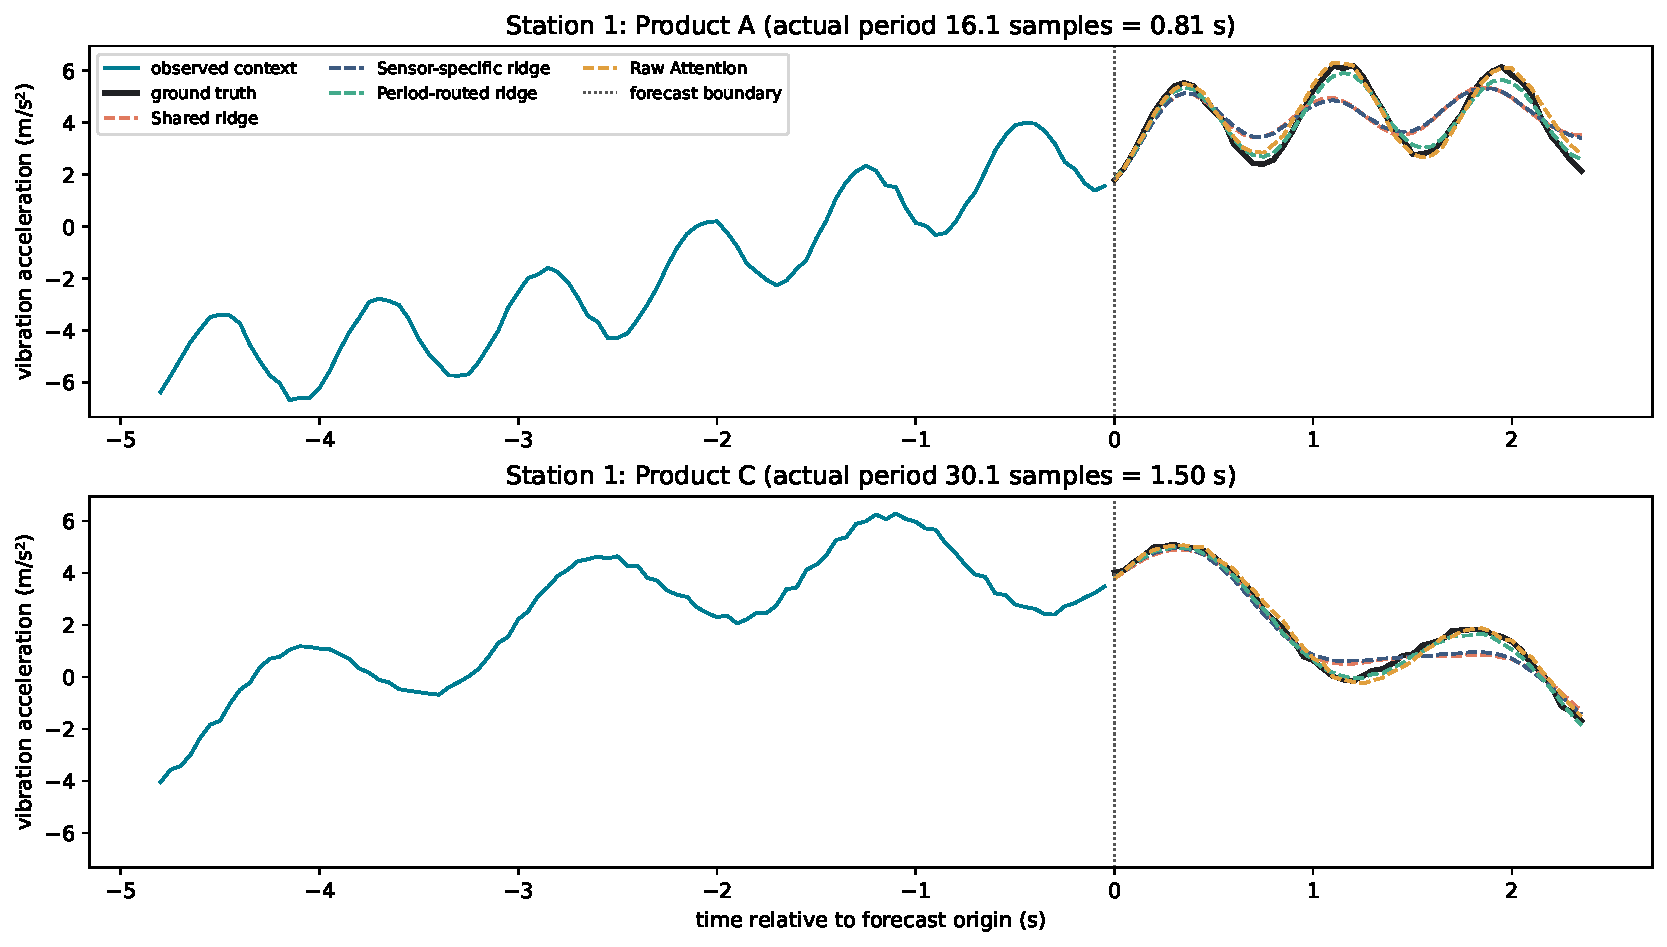
\includegraphics[width=0.85\linewidth]{figures/out1_2.pdf}
\caption{Output 1.2: Station 1 forecasts for Product A ($P=16.1$) and Product C ($P=30.1$).}
\end{figure}

\textbf{The compromise.} $\widehat W$ is one least-squares map over all paces. It has no input that
selects the right phase advance, so it predicts the pace-averaged continuation. Averaging
out-of-phase cycles shrinks amplitude:
\begin{itemize}
  \item Product A: the forecast peaks at about 5.0 vs a true 6.2 (window RMSE 0.779 vs 0.232 for
  period routing).
  \item Product C: the second hump is halved, about 0.9 vs 1.8 (0.448 vs 0.150).
\end{itemize}

\begin{figure}[h]\centering
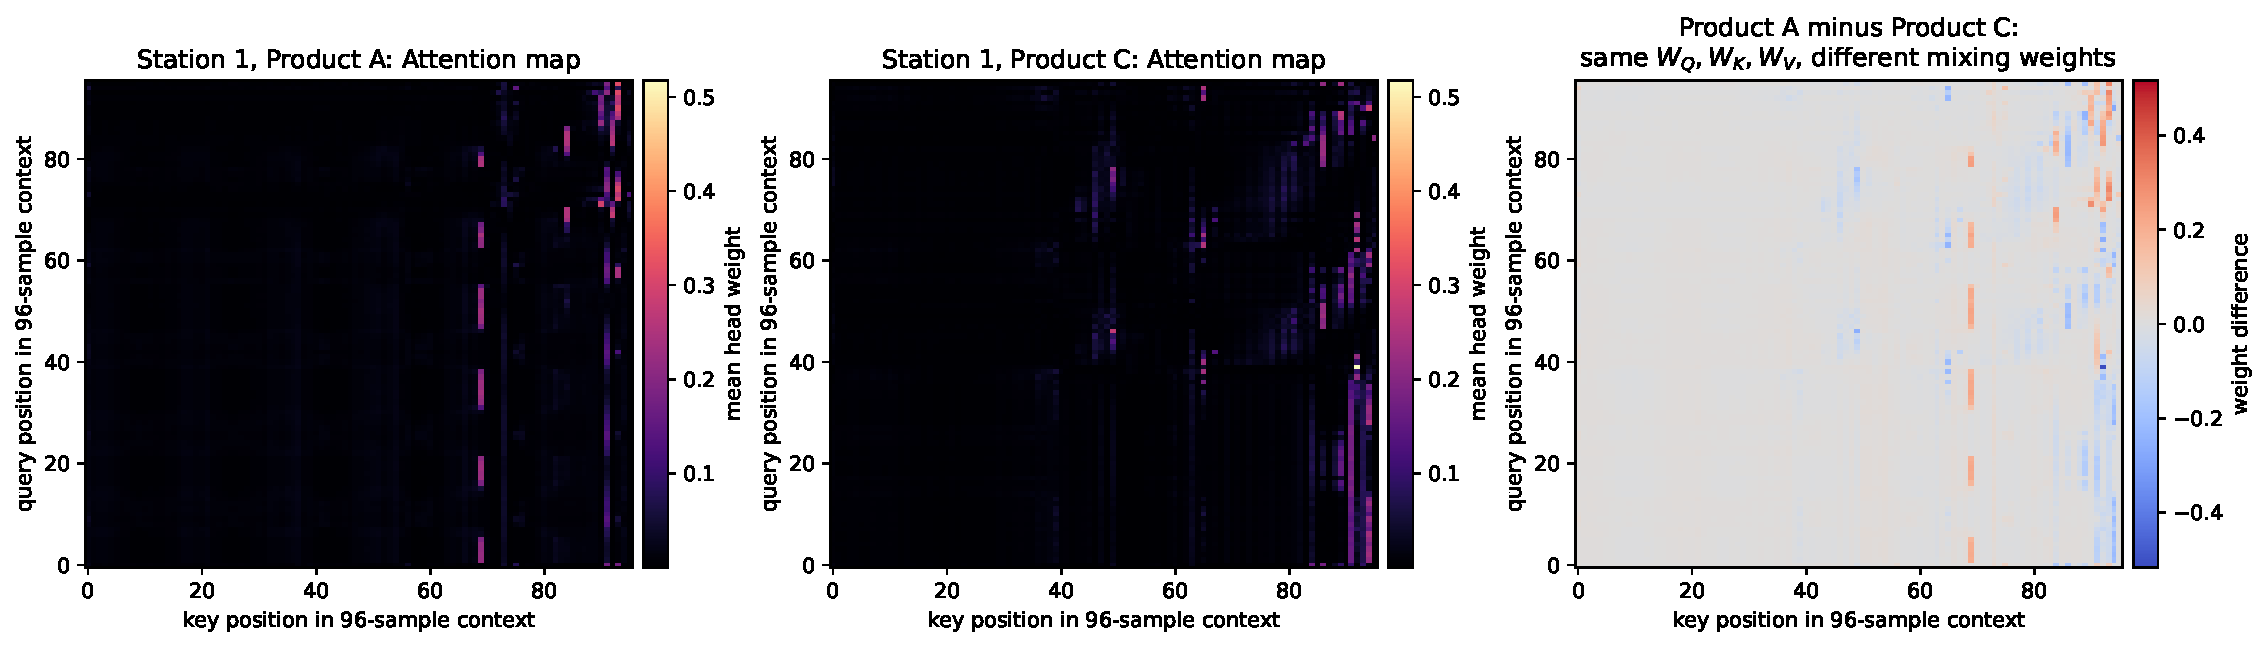
\includegraphics[width=\linewidth]{figures/out1_3.pdf}
\caption{Output 1.3: attention maps for the Product A and C contexts and their difference.}
\end{figure}

\textbf{Context-built mixing.} With the same frozen $W_Q,W_K,W_V$:
\begin{itemize}
  \item the A map focuses on key 69 and the last keys, while the C map spreads over keys 40--95;
  \item weights differ by up to 0.52.
\end{itemize}
Because $Q=XW_Q$ and $K=XW_K$, a new context changes $\mathrm{softmax}(QK^\top/\sqrt{d_h})$ and
therefore the mixing operator. Ridge applies one fixed $\widehat W$ to every input. This shows
context dependence, not period recovery.

%---------------------------------------------------------------------
\subsection*{Response 2}

\begin{figure}[h]\centering
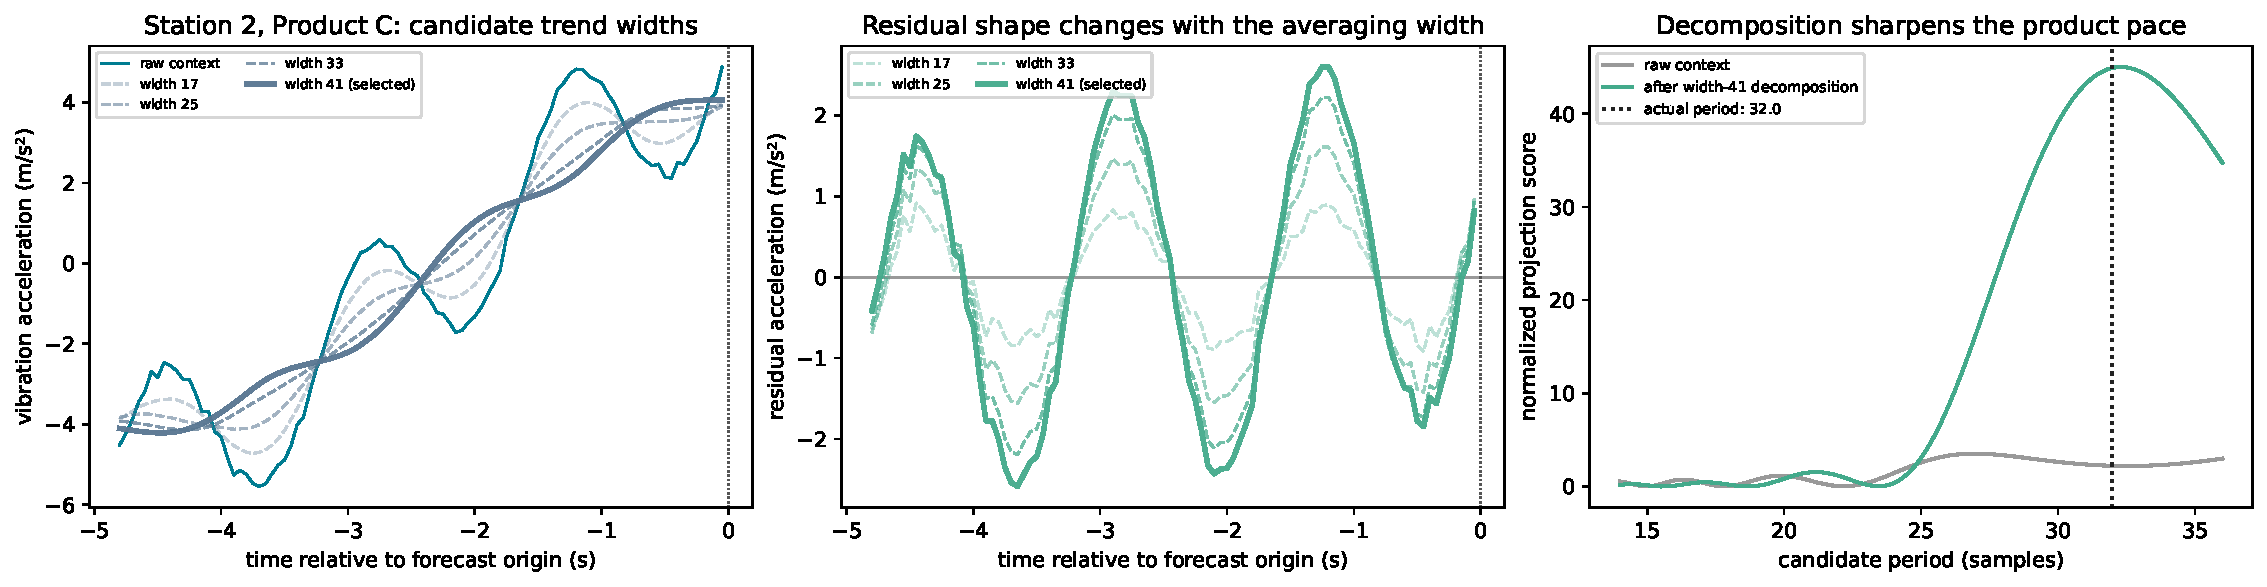
\includegraphics[width=\linewidth]{figures/out2_1.pdf}
\caption{Output 2.1: trend and residual for candidate widths (Station 2, Product C, $P=32$).}
\end{figure}

\textbf{Selected width: $m=41$.}
\begin{itemize}
  \item \textbf{Visual (2.1).} Small widths leave vibration in the trend. At $m=41$ the trend is a
  smooth ramp and the residual is a clean cycle (std $0.58\to1.57\ms$). The period score peaks
  sharply at the true $P=32$ only after decomposition.
  \item \textbf{Oracle (2.2).} Period recovery within one sample rises from 0.687 (raw) to 0.980
  ($m=17$) and 0.998 ($m=41$).
  \item \textbf{Ablation (2.3).} Raw Attention $0.421\to0.287$ established ($-32\%$) and
  $0.608\to0.428$ held-out ($-30\%$). The gain is largest on steep-ramp contexts.
\end{itemize}

\begin{figure}[h]\centering
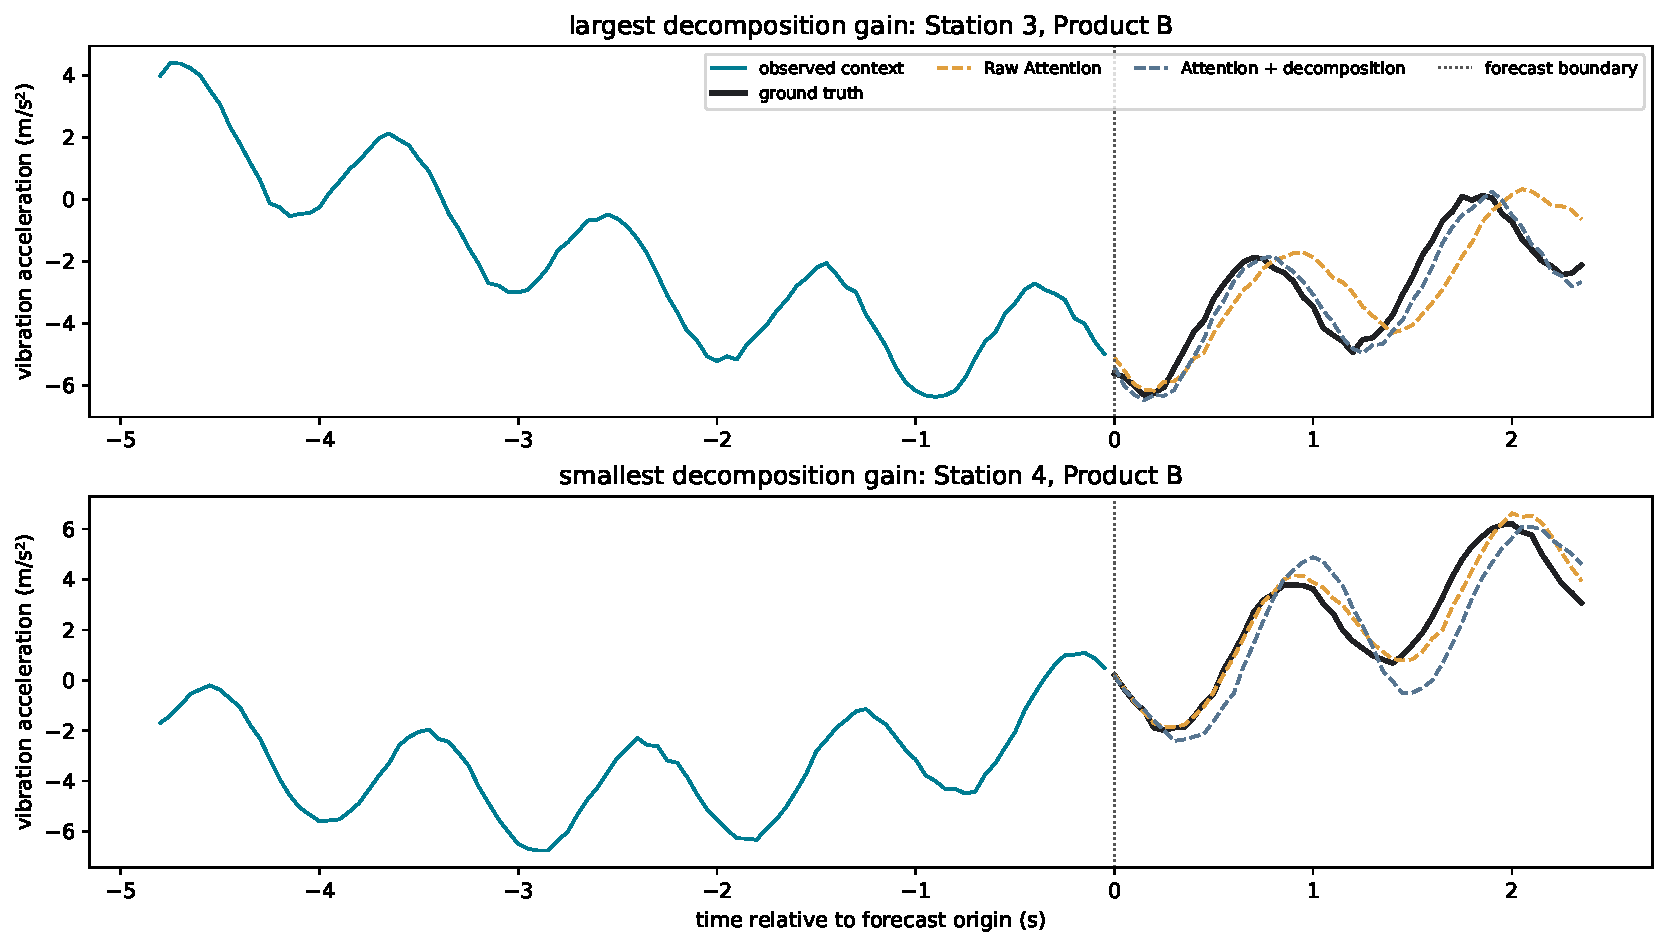
\includegraphics[width=0.8\linewidth]{figures/out2_3.pdf}
\caption{Output 2.3: largest gain on a steep ramp (top), smallest on a flat context (bottom).}
\end{figure}

\textbf{Why a moving average fits.} Drift ($\sim$240 samples) and vibration (14--36) have separated
time scales. A centered average longer than $P$ removes the cycle and keeps the near-linear drift.
The parameter-free filter cannot overfit station drift, which matches the held-out gain.

\textbf{Why the oracle diagnostic.} It measures directly what $m$ should achieve (exposing the
period). It uses the true period only to score widths on training windows, so there is no leakage.

\textbf{Failure case.} An abrupt level shift is smeared into a ramp and leaves a false bump in $S$.
A median filter or STL would preserve jumps and curvature, at the cost of more hyperparameters.

%---------------------------------------------------------------------
\subsection*{Response 3}

\textbf{Verification.}
\begin{itemize}
  \item The worked example gives $z=[35,15,25,25]$, as expected, confirming that delays look back.
  \item \texttt{delay\_scores} matches direct correlation ($4,-4,4,-4$).
\end{itemize}

\begin{figure}[h]\centering
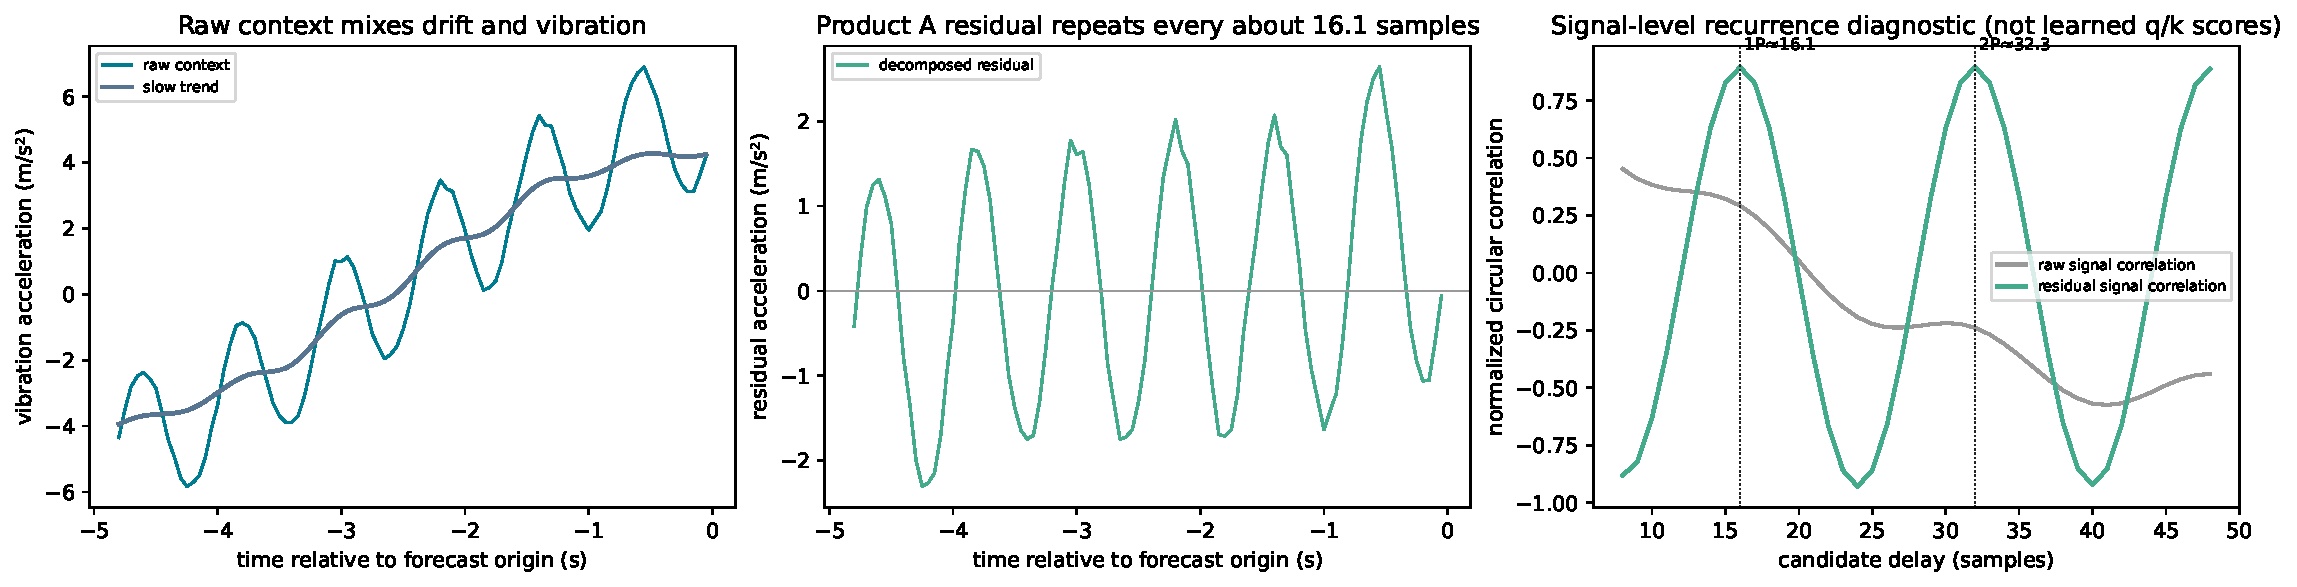
\includegraphics[width=\linewidth]{figures/out3_2.pdf}
\caption{Output 3.2: raw vs residual recurrence (Station 2, Product A, $P=16.1$).}
\end{figure}

\textbf{Strongest lags.}
\begin{itemize}
  \item Residual correlation peaks at $\tau=16$ (0.896) and $\tau=32$ (0.897), i.e.\ $P$ and $2P$.
  \item Troughs fall at half-period offsets (24, 40).
  \item A periodic signal recurs at every multiple of $P$, so blending these lags is safe.
\end{itemize}

\textbf{Why decomposition helps.} The raw correlation follows the ramp: it is high at short lags and
falls steadily, with no peak at $P$. Removing drift leaves a zero-mean cycle that correlates only
when peaks align. Useful structure is then a few shared displacements, which is exactly what the
delay mixer models with $L$ scores instead of $L^2$.

\textbf{Failure case.} If the period drifts within the context (e.g.\ 14 to 20 samples), no single
lag aligns the whole window. Blending mismatched lags cancels the cycle and damps the forecast.
Isolated spikes also fail, because circular shifts create false echoes.

%---------------------------------------------------------------------
\subsection*{Response 4}

\textbf{(a) Prediction}: decomposition should help most when drift
is prominent, because it hands the ramp to a linear head before mixing.

\textbf{(b) Results.}

\begin{table}[h]\centering\small
\begin{tabular}{lrrrrrr}
\toprule
Model & RMSE & MSE & St.\,4 RMSE & St.\,4 MSE & Params & Fit (s)\\
\midrule
Shared ridge & 0.767 & 0.588 & 0.876 & 0.767 & 4{,}608 & 0.002\\
Period-routed ridge & \textbf{0.166} & \textbf{0.028} & \textbf{0.173} & \textbf{0.030} & 59{,}904 & 0.002\\
Raw Attention & 0.421 & 0.178 & 0.608 & 0.369 & 368{,}368 & 802\\
Raw delay mixer & 0.224 & 0.050 & 0.337 & 0.113 & 368{,}370 & 1097\\
Attention + decomposition & 0.287 & 0.082 & 0.428 & 0.183 & 373{,}024 & 967\\
Autoformer-inspired & 0.198 & 0.039 & 0.240 & 0.057 & 373{,}026 & 1017\\
\bottomrule
\end{tabular}
\caption{Outputs 1.1 and 4.1: validation error and cost (established unless St.\,4).}
\end{table}

\begin{itemize}
  \item \textbf{Each switch helps alone.} MSE gain vs Raw Attention: delay mixing 0.128,
  decomposition 0.096.
  \item \textbf{Combined gain is 0.139, far below the 0.224 sum.} The switches overlap because both
  target drift plus repetition. The same holds on Station 4 (0.312 vs 0.442).
  \item \textbf{Prediction (a) was partly right.} Decomposition helped most on ramps, but delay
  mixing helped more overall.
  \item \textbf{Horizon (4.2).} Errors grow as phase errors accumulate. From $h=1$ to $h=48$:
  Raw Attention $0.149\to0.530$, Autoformer-inspired $0.135\to0.235$, period routing
  $0.112\to0.228$ (lowest throughout).
\end{itemize}

\begin{figure}[h]\centering
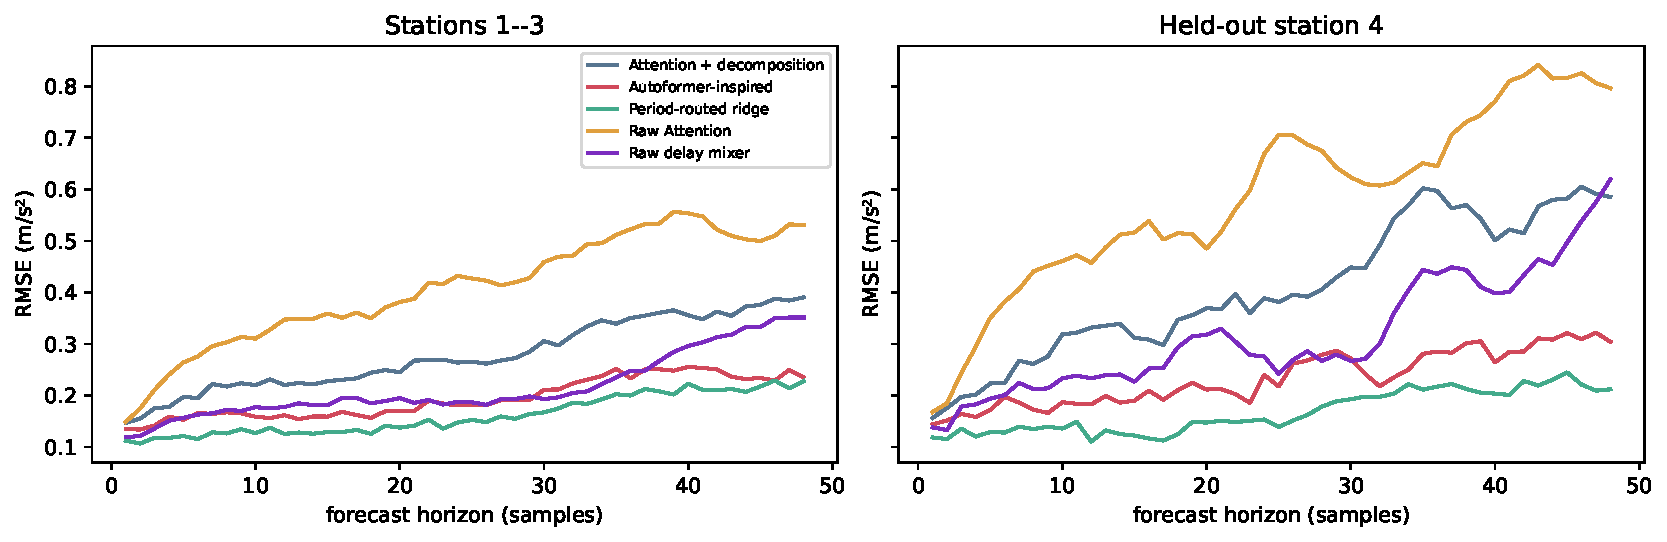
\includegraphics[width=0.85\linewidth]{figures/out4_2.pdf}
\caption{Output 4.2: RMSE along the 48-step horizon.}
\end{figure}

\textbf{(c) Deployment.} I chose \textbf{Period-routed ridge} for both populations, from validation
only:
\begin{itemize}
  \item Established: RMSE 0.166 vs 0.198 for the best neural model, $6\times$ fewer parameters,
  0.002\,s vs 1017\,s to fit.
  \item Station 4: RMSE 0.173 vs 0.240. It conditions on pace rather than station identity.
  \item Caveat: an unseen pace outside the routing bands would break it; Autoformer-inspired is the
  fallback.
  \item Test (Output 4.3): 0.161 established, 0.183 held-out.
\end{itemize}

\textbf{Interpretation.}
\begin{itemize}
  \item \textbf{The right inductive bias mattered more than flexibility.} A linear map routed by
  pace beat every Attention variant with $6\times$ fewer parameters, because it encodes the true
  cause directly.
  \item \textbf{The neural upgrades show the same lesson.} Decomposition and delay mixing each
  removed 30--50\% of Raw Attention's error at no parameter cost, but overlapped when combined.
  \item \textbf{Flexibility without bias generalised worst.} Raw Attention lost 44\% on Station 4.
  \item \textbf{Learned models pay off only where hand-built bias fails}, such as unseen paces.
\end{itemize}

\newpage
%=====================================================================
\section*{Task 2: Leaderboard Challenge}

\begin{table}[h]\centering\small
\begin{tabular}{ll}
\toprule
Model & Autoformer, 1 encoder + 1 decoder layer, $d=32$, future covariates\\
Parameters $P$ / epochs $E$ & 22{,}081 / 4\\
Validation RMSE (3 seeds) & $72.0\pm2.9$ (best baseline 112.0)\\
\textbf{Leaderboard RMSE / score} & \textbf{98.35 / 98.351 (rank 30, 1st attempt)}\\
Leaderboard MAE / sMAPE & 66.30 / 74.61\%\\
\bottomrule
\end{tabular}
\end{table}

Code: \texttt{Question 2 - Leaderboard/autoformer.py} (modes \texttt{ablate}, \texttt{final},
\texttt{figures}).

\subsection*{Data and preprocessing}
\begin{itemize}
  \item \textbf{Target.} Non-negative and heavy-tailed: mean 98, std 91, max 994. Autocorrelation
  decays fast (0.97 at lag 1, 0.40 at lag 24, 0.03 at lag 168).
  \item \textbf{Period.} The periodogram has sharp peaks at 24 and 12. I treat one step as one
  hour and add $\sin/\cos$ of $(\text{idx}\bmod24)$ as phase features (Fig.~\ref{fig:period}).
  \item \textbf{Covariates.} Six continuous variables (A--F) and a 4-way one-hot (G--J). A--C are
  z-scored; D--F are log-transformed then z-scored. Statistics use the training region only.
  \item \textbf{Scaling.} Global z-score of the target. Window-relative normalisation was avoided
  because absolute level carries signal (high levels tend to fall).
\end{itemize}

\begin{figure}[h]\centering
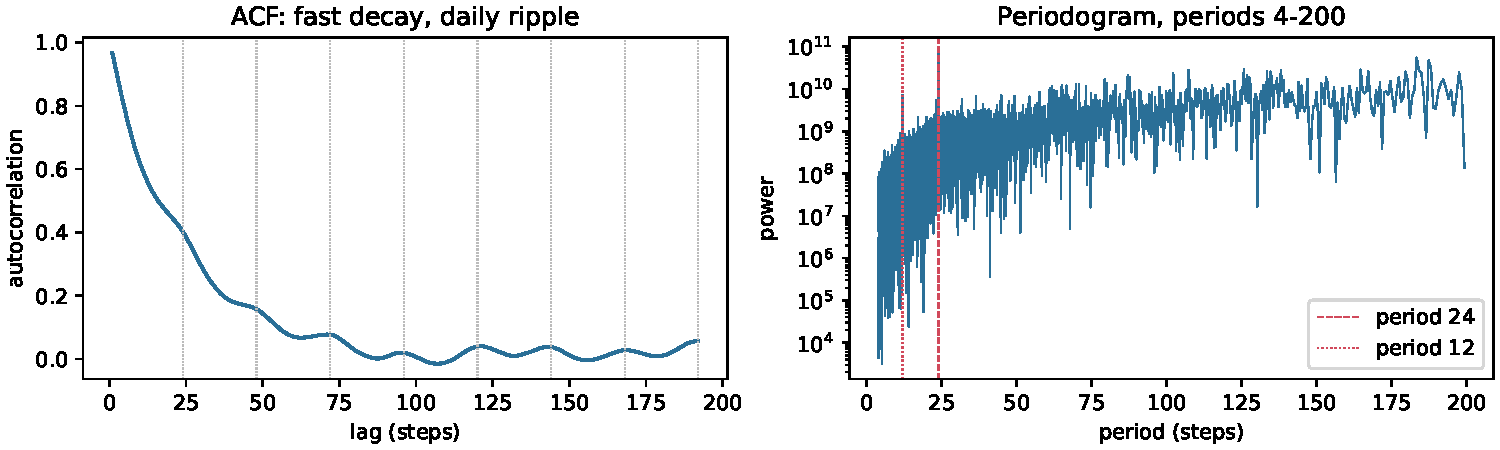
\includegraphics[width=0.85\linewidth]{figures/fig_periodicity.pdf}
\caption{Autocorrelation and periodogram of the training series: a 24-step cycle.}
\label{fig:period}
\end{figure}

\subsection*{Model}
Written in PyTorch, adapted from the official implementation:\\
\url{https://github.com/thuml/Autoformer}. It contains both required mechanisms:
\begin{itemize}
  \item \textbf{Series decomposition}: a moving average with kernel 25, applied at the input and
  after every sublayer. The decoder accumulates trend.
  \item \textbf{Auto-Correlation}: FFT delay scores, top $k=\lfloor\ln L\rfloor=5$ lags, and
  time-delay aggregation. It replaces dot-product attention in self- and cross-attention.
\end{itemize}
Covariates and phase enter as ``marks'' in both the encoder (past) and the decoder (horizon). Input
168, label 48, output 168.

\subsection*{Validation protocol}
\begin{itemize}
  \item \textbf{Chronological split.} The last 4{,}368 points form validation: 176 origins, each
  forecasting a full 168-step block. Training targets end before this region.
  \item \textbf{Training.} MSE loss, Adam ($10^{-3}$, halved each epoch), early stopping
  (patience 2). Each epoch sees every 4th window.
  \item \textbf{Seeds and metrics.} Three seeds per configuration; RMSE, MAE and sMAPE reported.
\end{itemize}

\subsection*{Ablation}

\begin{table}[h]\centering\small
\begin{tabular}{lccc}
\toprule
Configuration & RMSE (mean $\pm$ sd) & MAE & sMAPE (\%)\\
\midrule
Last-24h mean (best baseline) & 112.0 & 80.6 & 88.8\\
No covariates & $95.3\pm0.3$ & 72.4 & 81.1\\
No covariates, log target & $96.5\pm0.1$ & 67.6 & 82.9\\
Covariates, past only & $92.4\pm1.0$ & 70.2 & 80.1\\
\textbf{Covariates incl.\ horizon} & $\mathbf{72.0\pm2.9}$ & 54.6 & 71.7\\
Covariates incl.\ horizon, log target & $75.0\pm3.6$ & \textbf{48.8} & \textbf{59.4}\\
\bottomrule
\end{tabular}
\caption{Validation results, seeds 0--2.}
\end{table}

\begin{figure}[h]\centering
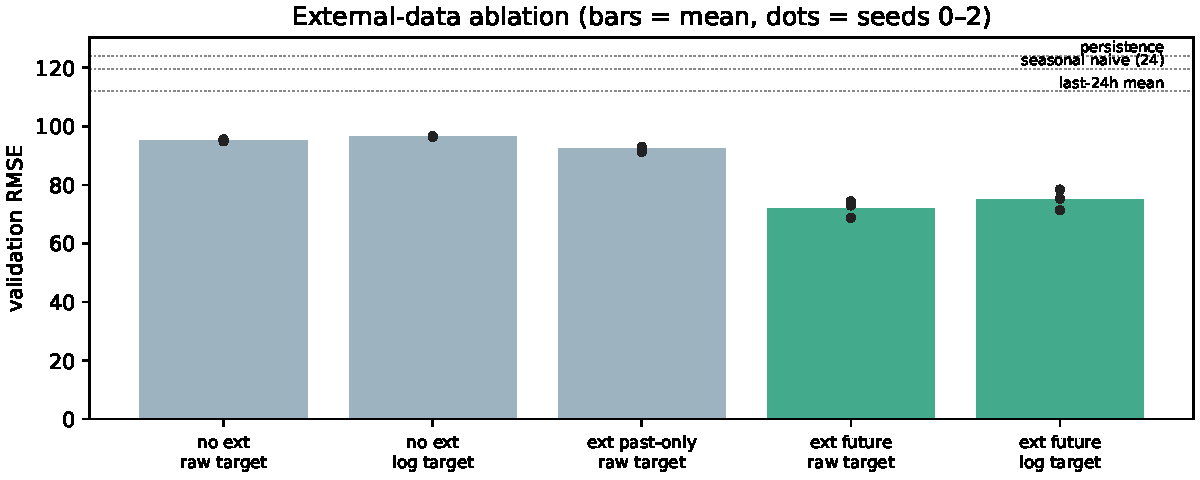
\includegraphics[width=0.8\linewidth]{figures/fig_ablation.pdf}
\caption{Ablation over seeds; dotted lines are baselines.}
\end{figure}

\begin{itemize}
  \item \textbf{Future covariates matter, past ones barely do.} Past-only covariates reduce RMSE by
  2.9; covariates over the horizon reduce it by 24\%, about $8\times$ the seed spread. Weather
  during the horizon decides whether the level builds or clears (Fig.~\ref{fig:valfc}).
  \item \textbf{Log target trades RMSE for MAE.} It improves MAE and sMAPE but underpredicts
  spikes, which dominate RMSE. Ranking uses RMSE, so I kept the raw target.
  \item \textbf{Final model.} Retrained from scratch on the full history with the best
  configuration, seed 0, $E=4$ (the mean best epoch).
\end{itemize}

\begin{figure}[h]\centering
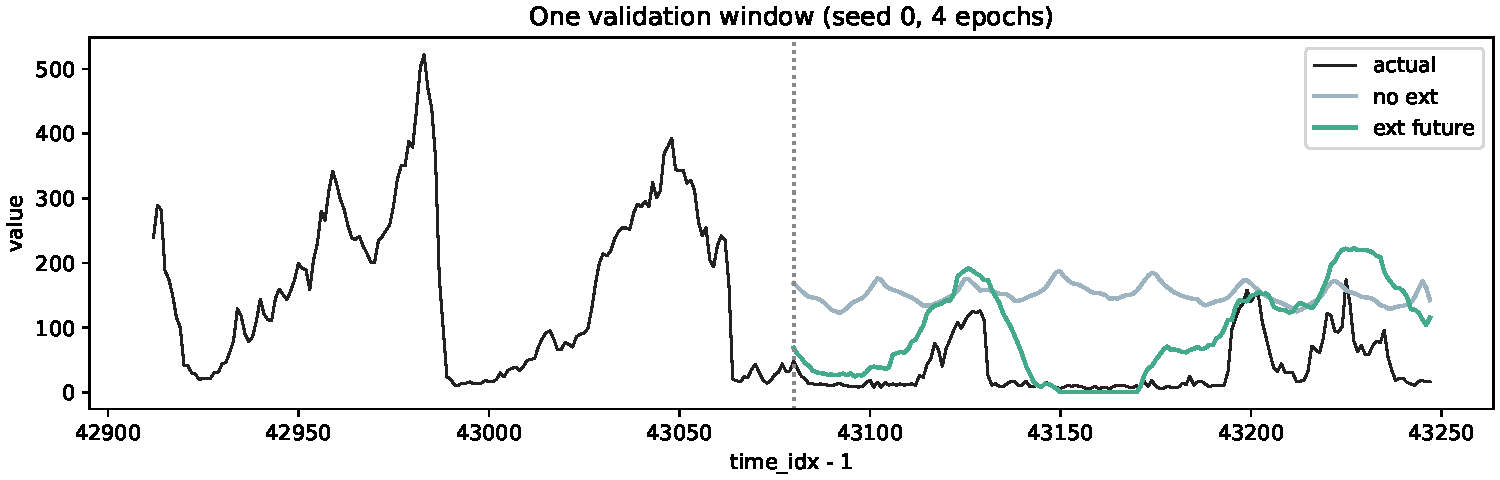
\includegraphics[width=\linewidth]{figures/fig_val_forecast.pdf}
\caption{One validation window. Horizon covariates let the model anticipate drops and rises.}
\label{fig:valfc}
\end{figure}

%=====================================================================
\section*{Use of Generative AI}
I used Claude Code (Anthropic, Claude Opus 5.5). 
I asked it to explain the Autoformer architecture and the series decomposition mechanism, and to summarize the differences between attention and auto-correlation. 
I used it to understand the tasks and how should I approach them.
I used it for scaffolding the tasks code and drafting the LaTeX report.

\section*{References}
\begin{itemize}
\item Wu et al.\ (2021). Autoformer: Decomposition Transformers with Auto-Correlation for Long-Term
Series Forecasting. NeurIPS. Code: \url{https://github.com/thuml/Autoformer}.
\item Vaswani et al.\ (2017). Attention Is All You Need. NeurIPS.
\item Zeng et al.\ (2023). Are Transformers Effective for Time Series Forecasting? AAAI.
\end{itemize}

\end{document}
